Here we will be testing the following versions of the SG-t-SNE-Pi algorithm:
\begin{itemize}
    \item The original C/C++ implementation of the SG-t-SNE-Pi algorithm.
    \item The pure Julia implementation of the SG-t-SNE-Pi algorithm before the modifications.
\end{itemize}
All the tests where performed on the same machine with the following specifications:
\begin{itemize}
    \item CPU: Intel Core i5-4460 @ 3.20GHz
    \item RAM: 16GB DDR3 787MHz
    \item OS: WSL 2 on Windows 10 Pro 64-bit
    \item Julia version: 1.10.0
\end{itemize}
The P matrix used for our results was set in a pseudo-random manner to ensure reproducibility. The parameters
used can be summed up in the following Julia code:
\begin{minted}[breaklines,escapeinside=||,
                mathescape=true, 
                linenos, 
                numbersep=3pt, 
                gobble=2, 
                frame=lines, 
                fontsize=\small, 
                framesep=2mm]{julia} 
    n = 1000;   # number of points
    d = 10;     # average degree
    
    # Set the random seed for reproducibility
    Random.seed!(42)
    
    # Generate the sparse matrix with a deterministic random pattern
    P = sprand(n, n, d/n)

    # Benchmark the sgtsnepi function
    results=[]
    for i in 1:20
        t=@elapsed SGtSNEpi.embed( P )
        push!(results,t)
    end
\end{minted}
The results of the benchmarks are shown in the following graphs:
\begin{figure}[H]
    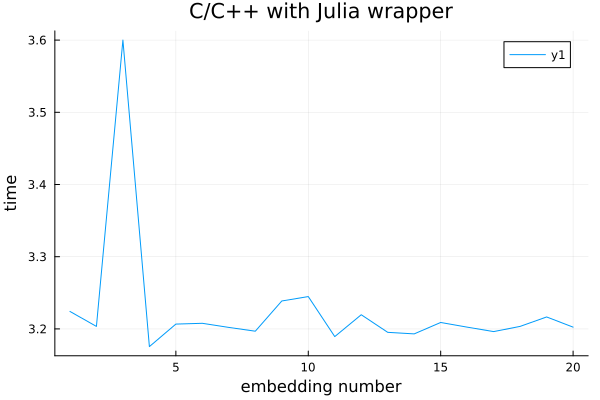
\includegraphics[width=0.5\textwidth]{media/c-c++plot.png}
    \caption{C/C++ with Julia wrapper}
\end{figure}
\begin{figure}[H]
    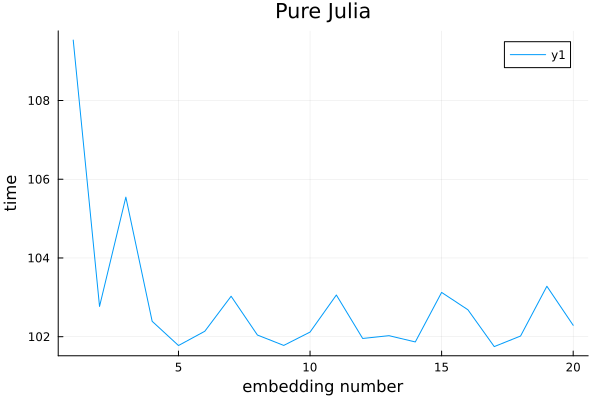
\includegraphics[width=0.5\textwidth]{media/embed.png}
    \caption{Pure Julia}
\end{figure}